\subsection{Long-range number-units}
To successfully perform the NA-task, the LSTM network should encode and store the grammatical number of the subject up to one step before the verb, when prediction of the verb form (singular or plural) occurs. In some cases, this may be quite challenging, in particular in the case of a long-range dependency between subject and verb, and when another noun with an opposite number appears before the verb (cite and cite). This section explores the underlying mechanism that enables the network to encode and store number information in various syntactic constructions, including those with such interfering nouns. The section has the following structure: subsection 5.1.1 describes an ablation study, which reveals \textit{long-range number units (LR-number units)} that can store and carry number information from subject to verb across interfering noun. Then, subsection 5.1.2 describes in details the gating and state dynamics of the identified LR-number units during the processing of sentences with long-range dependencies. Finally, subsection 5.1.3 explores the structure of the efferent weights of LR-number units that project onto the output layer.

\subsubsection{Local vs. distributed code - an ablation study}
Generally, number information may be stored in the network in either a local, sparse, or a distributed way, depending on the fraction of active units that carry this information. We hypothesized that if the network uses a local or sparse coding, meaning that there's a small set of units that encode number information, then ablating these units would lead to a drastic decrease in performance on the NA-task, compared to when ablating other units. To test this, we conducted ablation experiments in which each time a single unit of the network is ablated and the resulting model is then evaluated on several NA-tasks. Each NA-task contained sentences with a fixed syntactic structure, such as "Det Noun Adv Verb" or "Det Noun P Det Noun Verb", and each task was composed of several conditions depending on the possible assignments of grammatical number to the nonu(s) in the sentence. In addition, we also evaluated each ablated model on the Linzen task (see section 3.1 for details about all NA-tasks). Tables 1-2 summarize the results of all ablation experiments, showing units whose ablation resulted in a performance decrease of more than 10\% (TODO: choose a non-arbitrary threshold by looking at the distribution across all experiments - mean + 3sd for example). For each NA-task, the performance of the non-ablated model is also reported.

\begin{table}[h!]
\centering
\begin{tabular}{|P{2cm}||P{2cm}|P{2cm}|}
\hline
\B NA-task & \B N1-singular & \B N1-plural \\
\hline
\hline
\B Simple & 100\% & 100\% \\
\B Single-adv & 100\% & 99.56\% \\
\B Two-adv & 99.78\% & 99\% \\
\B name-PP & 98.89\% & 66.78\% \\
770 & - & 81.45 \\
776 & - & 57.58\% \\
848 & - & 87.6\% \\
\B adv-conj & 98.83\% & 99.67\% \\ 
988 & 83.98\% & - \\
1283 & 83.98\% & - \\
776 & - & 78.89\% \\
\hline
\end{tabular}
\caption{Ablation results: Percentage of correct subject-verb agreements in the two conditions of the NA-tasks (section 3.1). (? remove percentage sign from all ? )}
\end{table}

\begin{table}[h!]
\centering
\begin{tabular}{|P{1.8cm}||P{1cm}|P{1cm}|P{1cm}|P{1cm}|}
 \hline
\B NA-task & \B SS & \B SP & \B PS & \B PP\\
\hline
\hline
\B with-PP & 97.5\% & 88.5\% & 93.2\% & 98.3\% \\
770 & - & 89.8\% & 85.2\% & - \\
776 & - & - & 49.7\% & 81.7\% \\
988 & - & 58.76\% & - & - \\
\B subjrel & & & & \\

\B objrel & 64.67\% & 45.67\% & 69\% & 81\%\\
250 & 74.7\% & 67.9\% & - & - \\
309 & - & 83.6\% & - & - \\
495 & 84.0\% & 79.6\% & - & - \\
770 & 88.9\% & 82.8\% & 87.7\% & - \\
776 & - & - & 89.9\% & - \\
1150 & - & 76.3\% & - & - \\
\hline
\end{tabular}
\caption{Ablation results: Percentage of correct subject-verb agreements in NA-tasks with two nouns before the verb: SS - singular-singular, SP - singular-plural, PS - plural-singular, PP - plural-plural}
\end{table}


We highlight several important aspects of these results. First, in all NA-tasks, only a handful of units in the entire network (1300 units) had a significant effect on task performance. This results suggests a local, or sparse coding scheme for long-range grammatical-number information (TODO: quantify 'significant' reduction, and 'sparseness' of the code). Units that had highest effect are: 775, 987, 1282, 769, ... Second, for several tasks, such as the simple NA-task, none of the units had a signifcant effect on performance. This result suggests that number information is encoded and stored locally only for long-range dependencies, but that for short-range dependencies number information may still be encoded in other units, in a more distributed way (TODO: perhaps run a regression/classifier model to decode 'transient' number information as opposed to 'stored' one from the newtork, or use for this the results from the classifier in the generalization-across-time). We therefore distinguish between long-range (LR) number and short-range (SR) number units. Third, some units have an effect that depends on the grammatical number of the noun. For example, in the with-PP NA-task, ablating unit 987 had a signficant effect only when the first noun was singular, but not plural. This suggest that LR-number units should be further distinguished into \textit{LR-singular-number} and \textit{LR-plural-number units}. For example, unit 987 is a LR-singular-number unit, or \textit{singular unit} in short. (TODO: quantify numerosity of a unit - whether it's a singualr or plural. What is the criterion for that?). Third, Some NA-tasks and conditions are clearly more difficult to the network, even for the non-ablated model, as was previoulsy reported for humans and LSTM-LMs (cite and cite). For example, performance on the simple NA-task is greater than that on the with-PP NA-task, and the incongruent conditions SP and PS are more difficult to the network than the congurent conditions: SS and PP. We explore this point in more details in section 5.4. Finally, singular information was consistently more difficult to be reliably encoded for across long-distances compared to plural. This asymmetry was already reported for humans (cite Bock). However, in cotrast to phonological or morphological-based explanations suggested in this study, our results point to a cause residing at the work level, given that the LSTM-LM was trained on word tokens.


\subsubsection{Visualizing unit dynamics}
Having identified LR-number units, we now characterize the mechanism underlying grammatical-number information in these units. We examplify 

In particular, to carry number information from the subject to the verb, the forget gate of number units should be set to one during the entire period that separates them. 

For example, to carry number information from the subject to the verb, the forget-gate activity is likely to be close to one, whereas input-gate activity is likely to be non-zero only during the presentation time of the subject (Figure 1B). To explore this, we visualized gates and state dynamics of LR-number units during the processing of well-controlled sets of stimuli (section 3.1)

\begin{figure}[t]
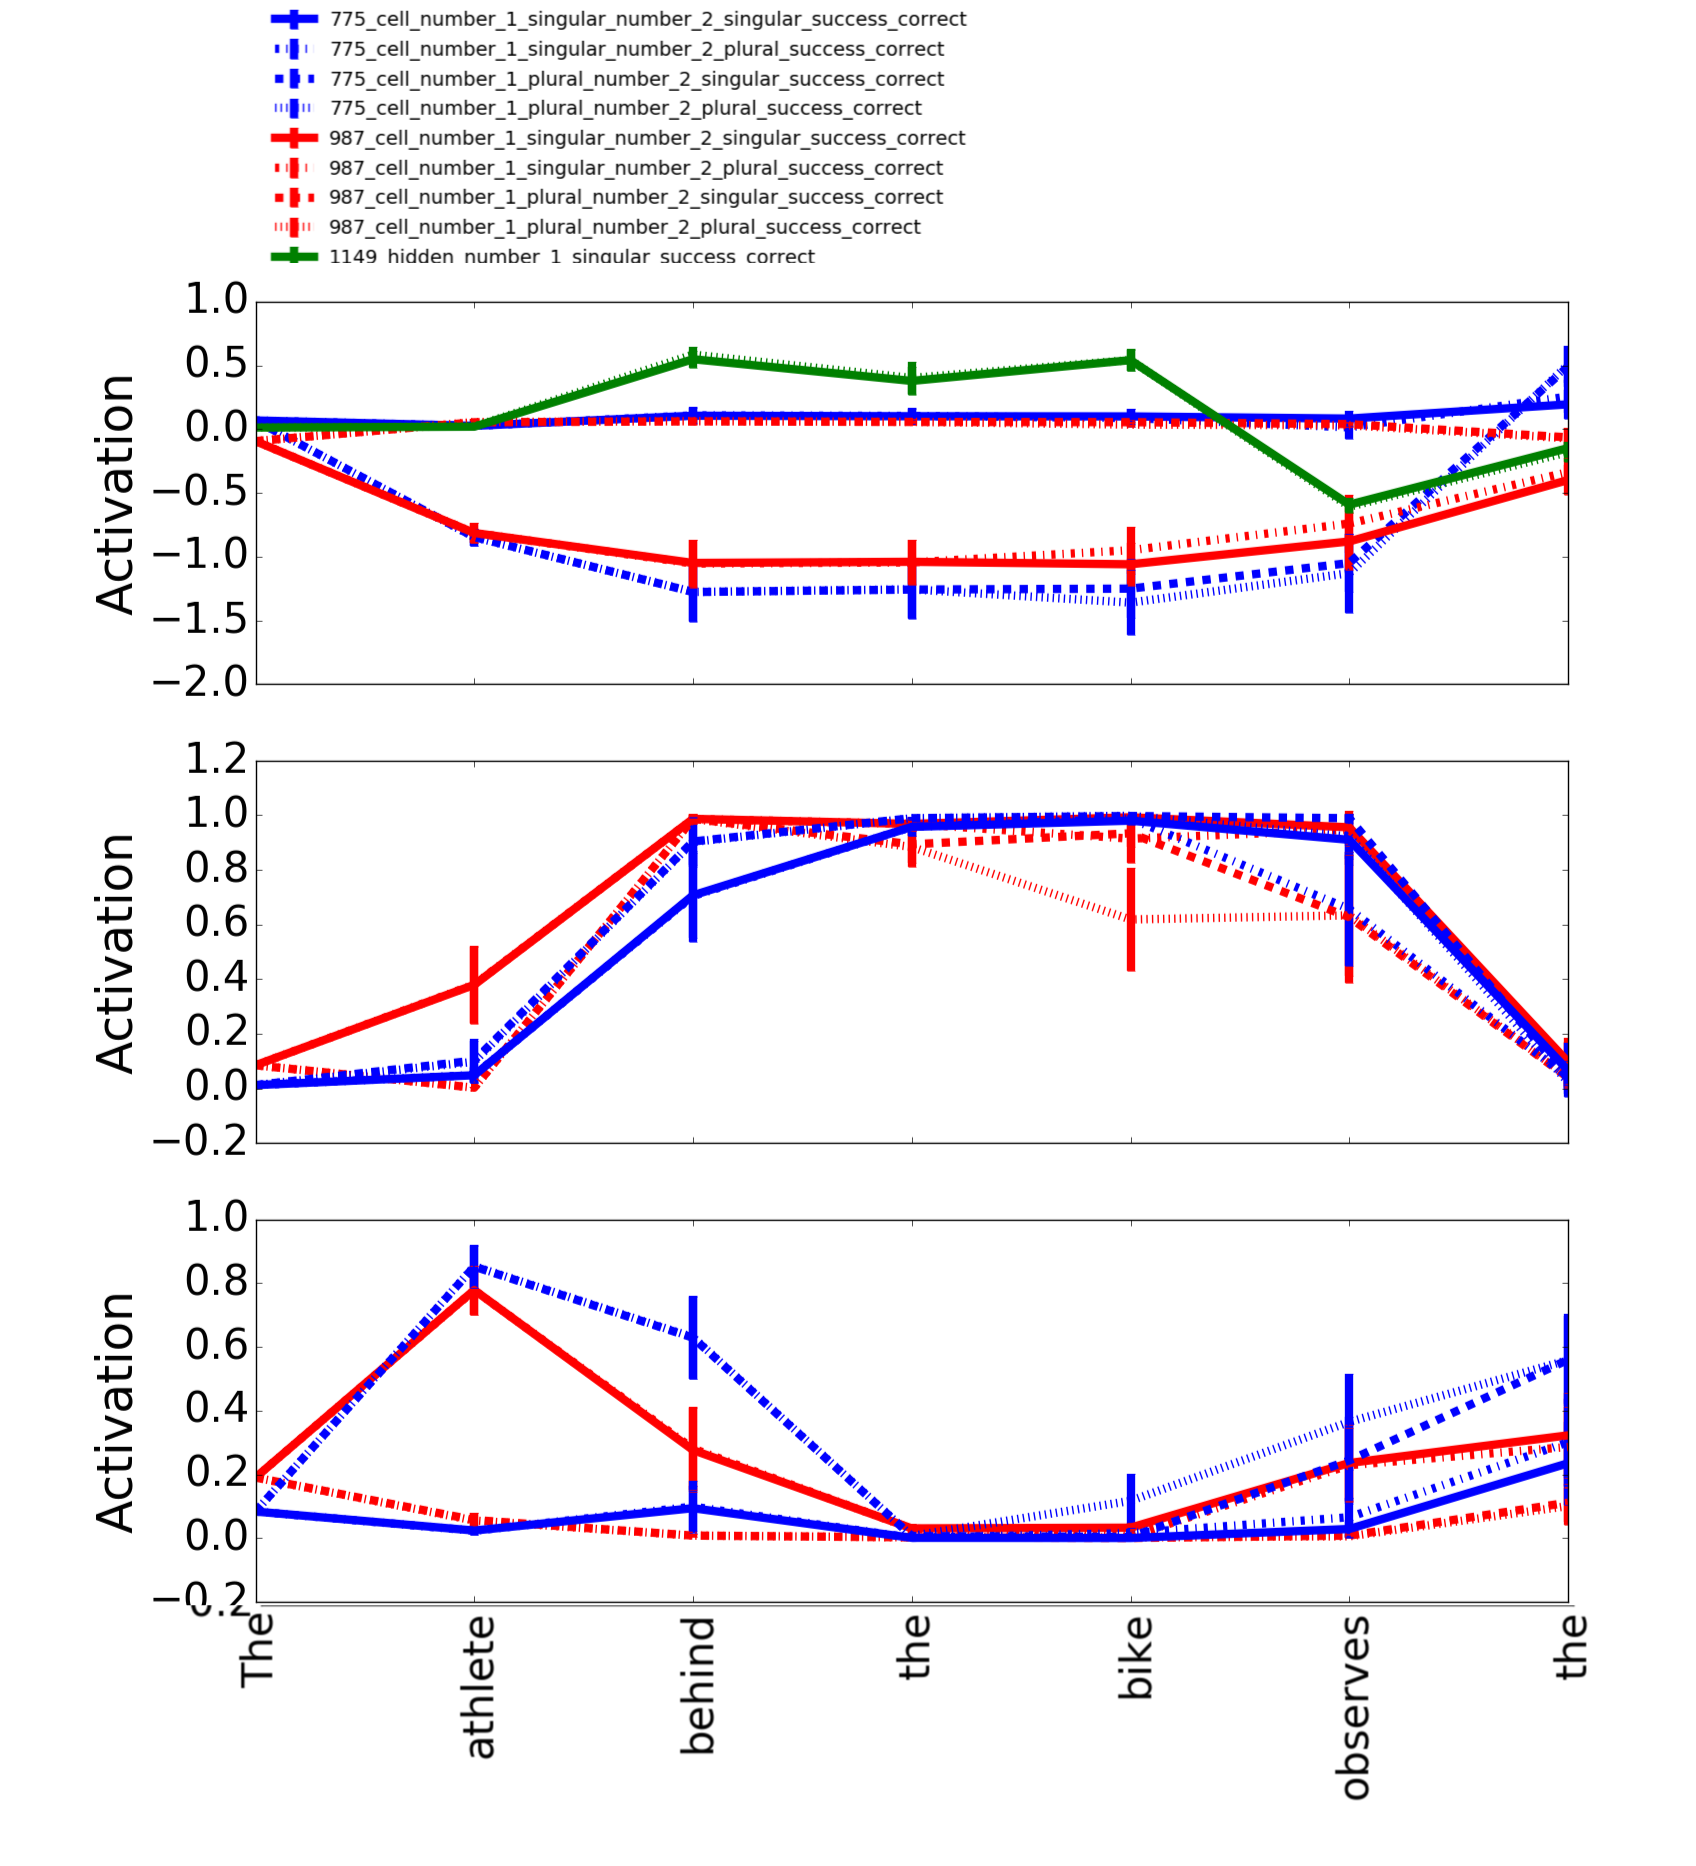
\includegraphics[width=\linewidth]{Figures/Figure2_number_units.png}
\caption{Cell and gate activations during processing of a sentence with a prepositional phrase between subject and verb. (A) Cell activity $C_t$ for the two number units 775 and 987 and output activity $h_t$ for the syntax unit 1149, for all four combinations of grammatical numbers of the two nouns. Note that the cell activity of units 775/987 is non-zero only when the first noun is plural/singular, respectively. (B) Corresponding forget-gate activity for the same number units. Note that gate activity is indifferent of the grammatical number of both nouns and that its value is close to one during the PP until after the verb. (C) Input-gate activity of the same units. Note that the gate value of unit 775/987 spikes around the first noun only when it is plural/singular.}
\end{figure}

\lipsum[1]

\begin{figure}
\centering
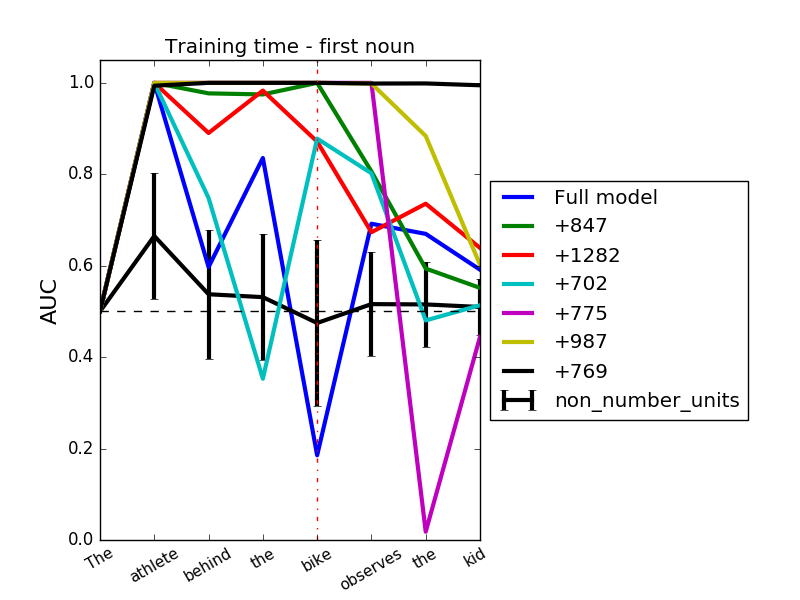
\includegraphics[width=\linewidth]{Figures/Figure3_number_units_GAT.png}
\caption{Generalization across time. To test whether the grammatical number of the first noun can be decoded from units activity at different time points, a linear-SVM was trained on unit activations $h_t$ at the time step of the first noun and then evaluated on all other time points. Area Under of Curve (AUC) values are shown for several cases: decoding from all LSTM units (full-model, black), a single number unit (775, purple; 1282, red...), average across all non-number units (black, error-bars represent standard-deviation). Note that the decoding of first-noun number is significantly higher from number units compared to all other units ($p-value<0.$).}
\end{figure}

\lipsum[1]

\subsubsection{Predicting the verb form}
Output weights + PCA
Section 5.1.2 summarizes these findings. Finally, to predict the proper verb form, number information should be projected from number units to the output layer. Section 5.1.3 explores the structure of the efferent weights of the number units. 

These efferent weights propagate grammatical-number information to the output layer, allowing for the prediction of the proper verb form (singular or plural). 

\begin{figure*}[t]
\centering
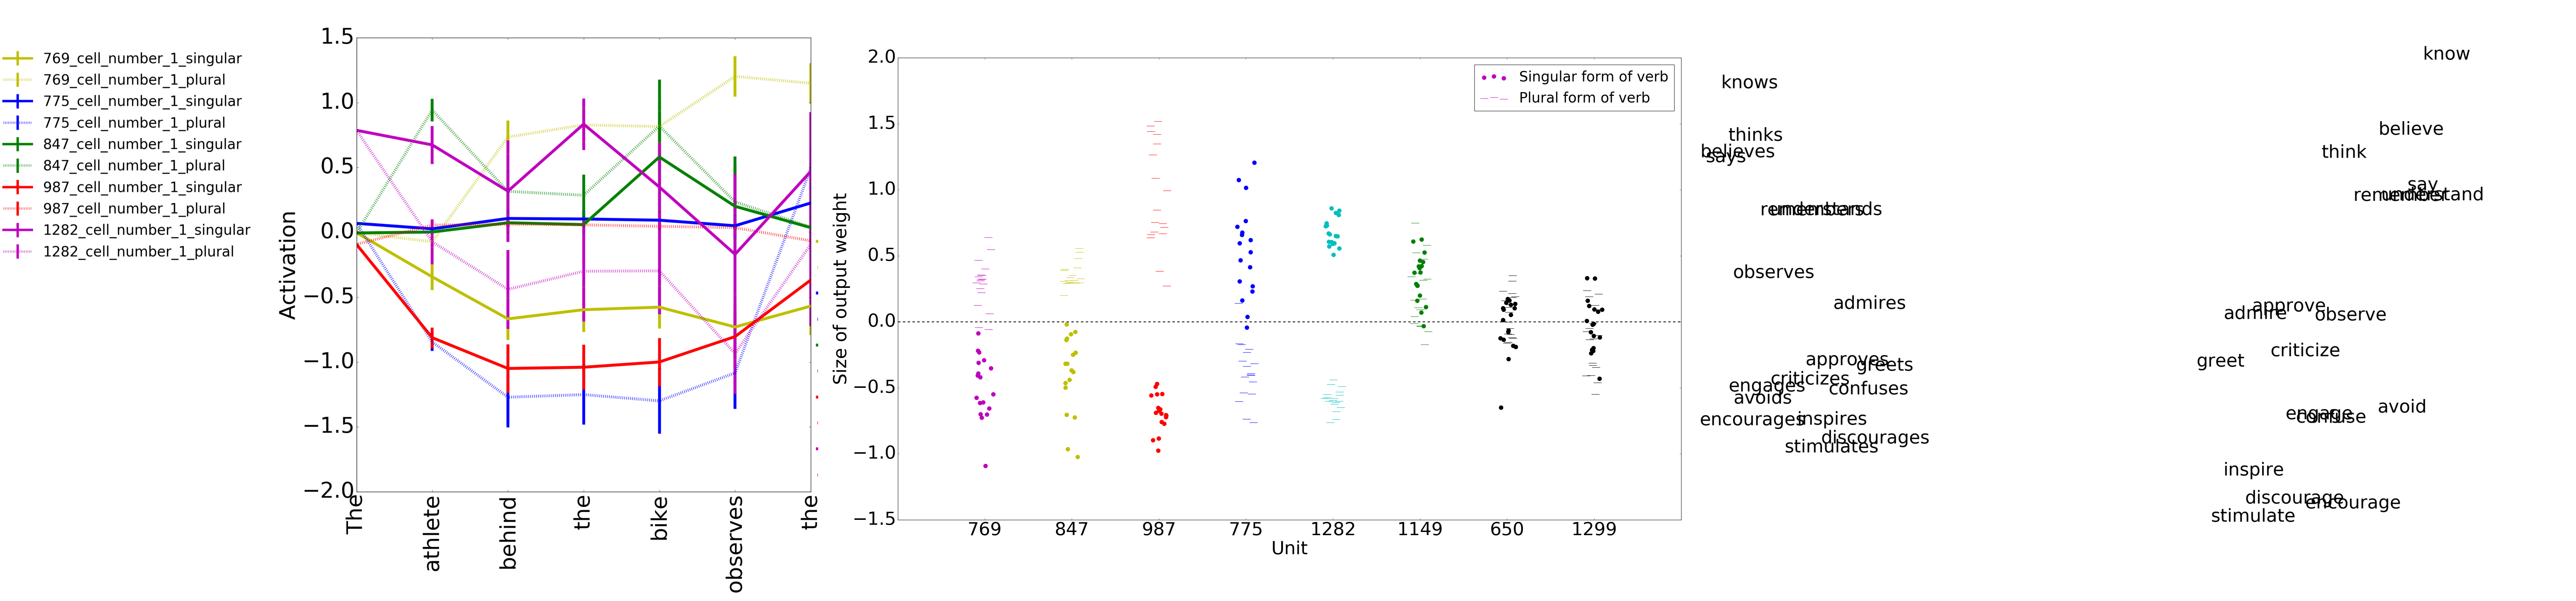
\includegraphics[width=\textwidth]{Figures/Figure4_output_weights.png}
\caption{Connectivity structure to output layer. (A) Output activity $h_t$ of all number units during the processing of a sentence with a PP between subject and verb. (B) Weight values from various units to output layer. Note that only for number units the output weights are clearly separated between singular and plural form of the verb, either positive or negative, compare to the syntax unit (1149) and two non-number units in the second layer. (C) Visualization of 18 verbs in their plural and singular forms (36 words in total) on the plane spanned by the two first principal components of their embeddings by the output weight matrix. A clear separation is observed between the singular and plural form along the first PC.}
\end{figure*}

\begin{figure}[b]
\centering
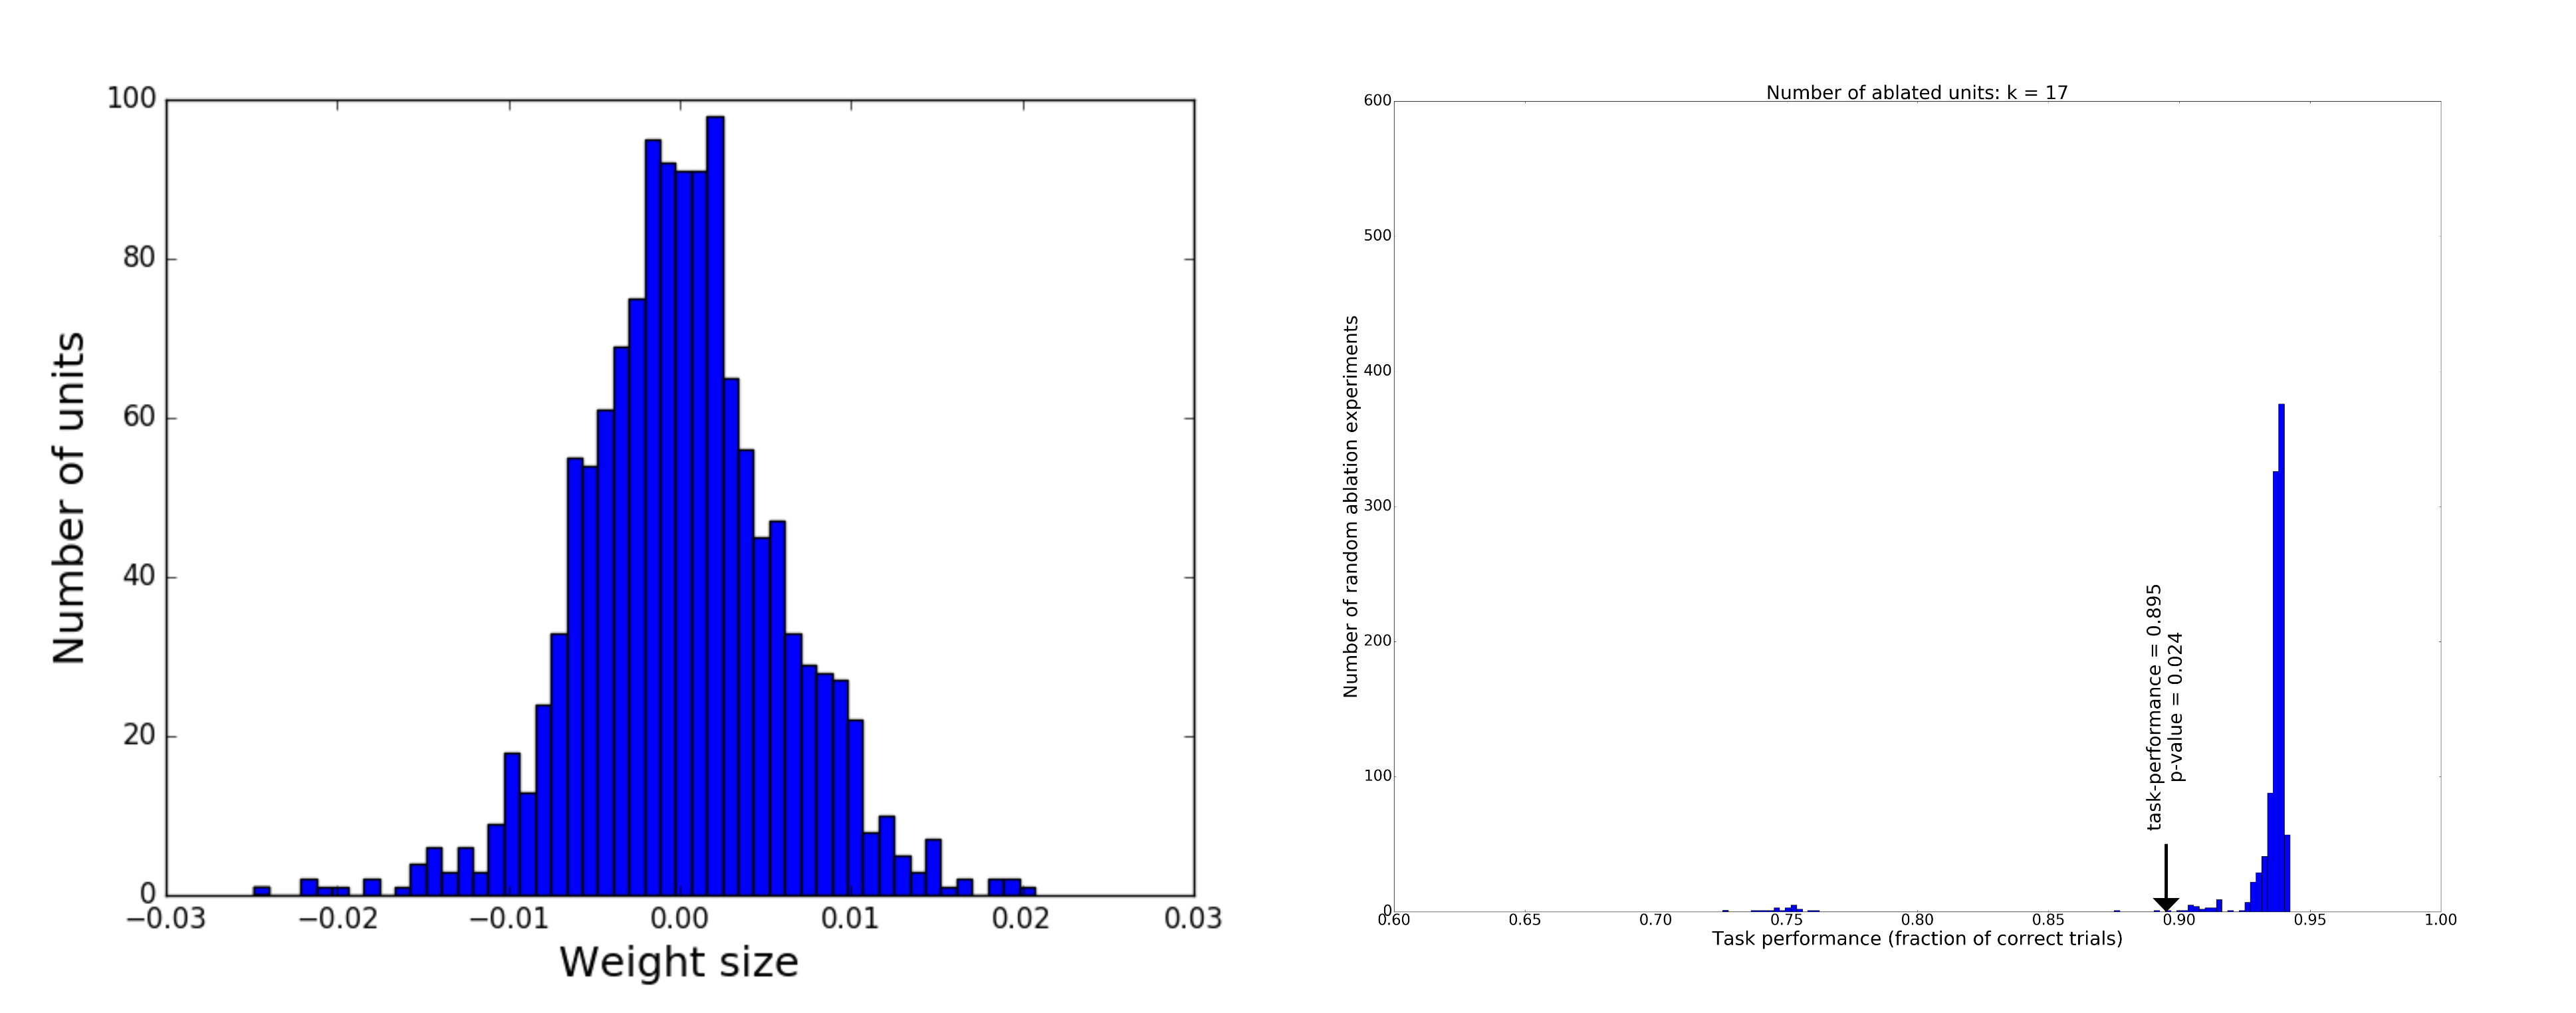
\includegraphics[width=\linewidth]{Figures/Figure6_regression.png}
\caption{(A) Distribution of the resulting weight values from the tree-depth regression model. Outlier weights were defined as having a value that is distant from the mean by more than three standard deviations (17 outlier weights in total - marked in red). (B) Task performance of 1000 models after ablating 17 random units (in blue) and based on the 17 outlier weights from the tree-depth regression model (black arrow). The reduction in performance due to outlier-weights ablation is statistically significant ($p-value < 0.05$) when compared to the null distribution generated by the random ablations.}
\end{figure}

